\section{\ExercisePrefixEmbeddedC Eigenes Microcontroller-Projekt umsetzen \optional}

Nachdem du einige der Ein- und Ausgabemöglichkeiten des Boards kennengelernt hast, besteht deine Aufgabe in diesem Teil darin, ein kleines Projekt deiner Wahl umzusetzen.
Du hast hierbei die freie Wahl, die folgenden Vorschläge sollen nur als Anregung dienen.

\subsection*{Vorschlag: Pong}
Zwei Gegner sollen je einen Balken (Rechteck) am linken oder rechten Rand des Spielfeldes mit den Schiebereglern steuern können, um einen Ball (ein Quadrat) im Spiel zu halten.
Erreicht der Ball den linken oder rechten Rand des Spielfelds, so bekommt der Spieler auf der anderen Seite einen Punkt und der Ball wird an seine Anfangsposition (die Mitte des Spielfelds) zurückversetzt.
Erreicht der Ball den oberen oder unteren Rand sowie einen der Balken der Spieler, so wird der Ball reflektiert - verlässt also niemals das Spielfeld.

Gewonnen hat der Spieler, der zuerst eine definierte Anzahl an Punkten erreicht.
Der aktuelle Punktestand könnte ebenfalls auf dem Display angezeigt werden.
\begin{center}
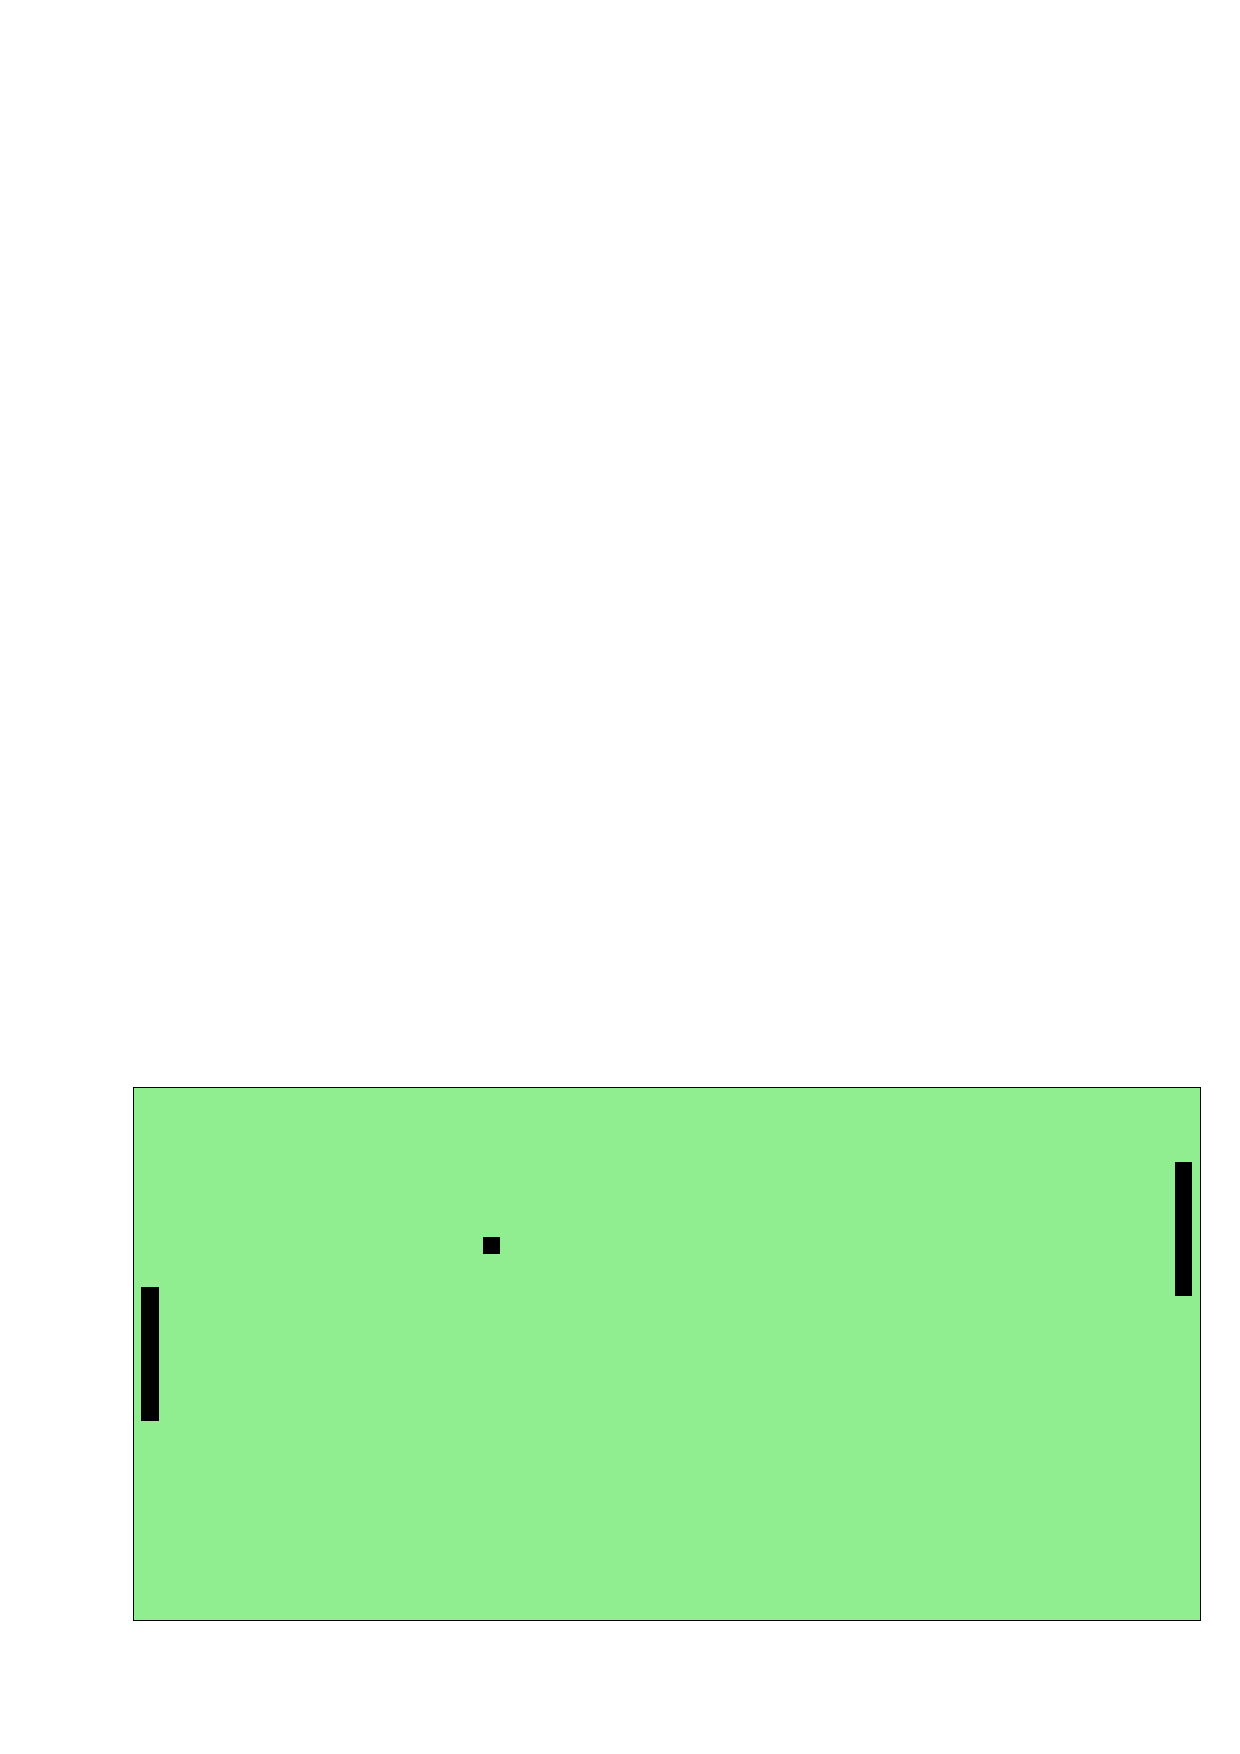
\includegraphics[scale=0.4]{05_c/figures/pong}
\end{center}



\subsection*{Vorschlag: Game of Life}
\glqq{}Game of Life\grqq{}\footnote{siehe auch \url{http://de.wikipedia.org/wiki/Conways_Spiel_des_Lebens}} besteht aus einem zweidimensionalen Spielfeld.
Jedes Feld steht für eine Zelle, die \textit{tot} oder \textit{lebendig} ist. Die Farben für den Zustand kannst du natürlich frei wählen.
Jede Zelle hat acht Nachbarzellen, die ebenso tot oder lebendig sein können.
Zu Beginn gibt es eine vordefinierte Anfangsgeneration.
Durch festgelegte Regeln wird die nachfolgende Generation ermittelt:
\begin{itemize}
	\item Eine \textbf{lebende Zelle} \dots
	\begin{itemize}
		\item mit 1 oder 0 lebenden Nachbarn stirbt aus Einsamkeit.
		\item mit 4 oder mehr lebenden Nachbarn stirbt wegen Übervölkerung.
		\item mit 2 oder 3 lebenden Nachbarn bleibt am Leben.
	\end{itemize}
	\item Eine \textbf{tote Zelle} mit genau 3 lebenden Nachbarn wird in der nächsten Generation geboren werden, andernfalls bleibt sie tot.
\end{itemize}
%
Als Anfangsgeneration eignen sich zufällige Populationen oder eine der folgenden Figuren:
\begin{center}
	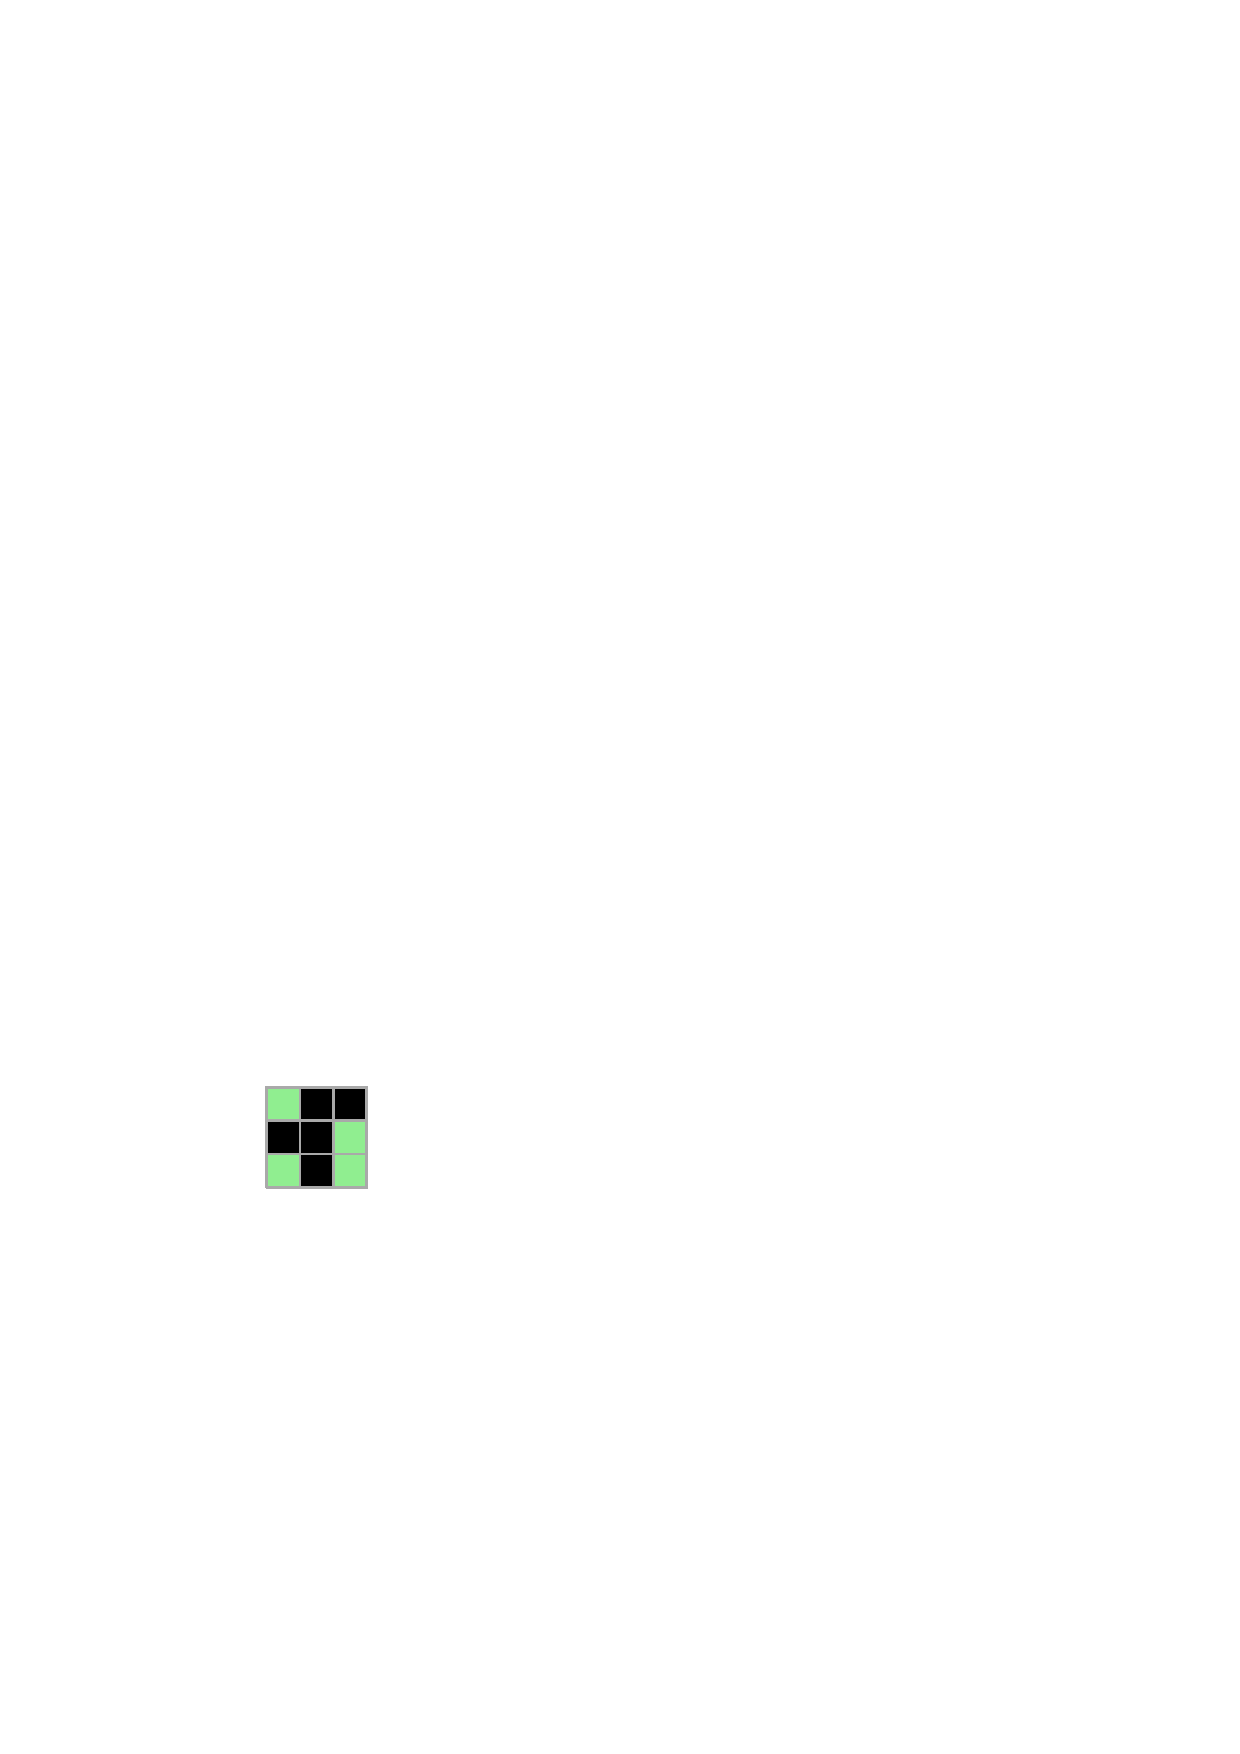
\includegraphics[scale=1]{05_c/figures/gol_init1}
	\hspace{5mm}
	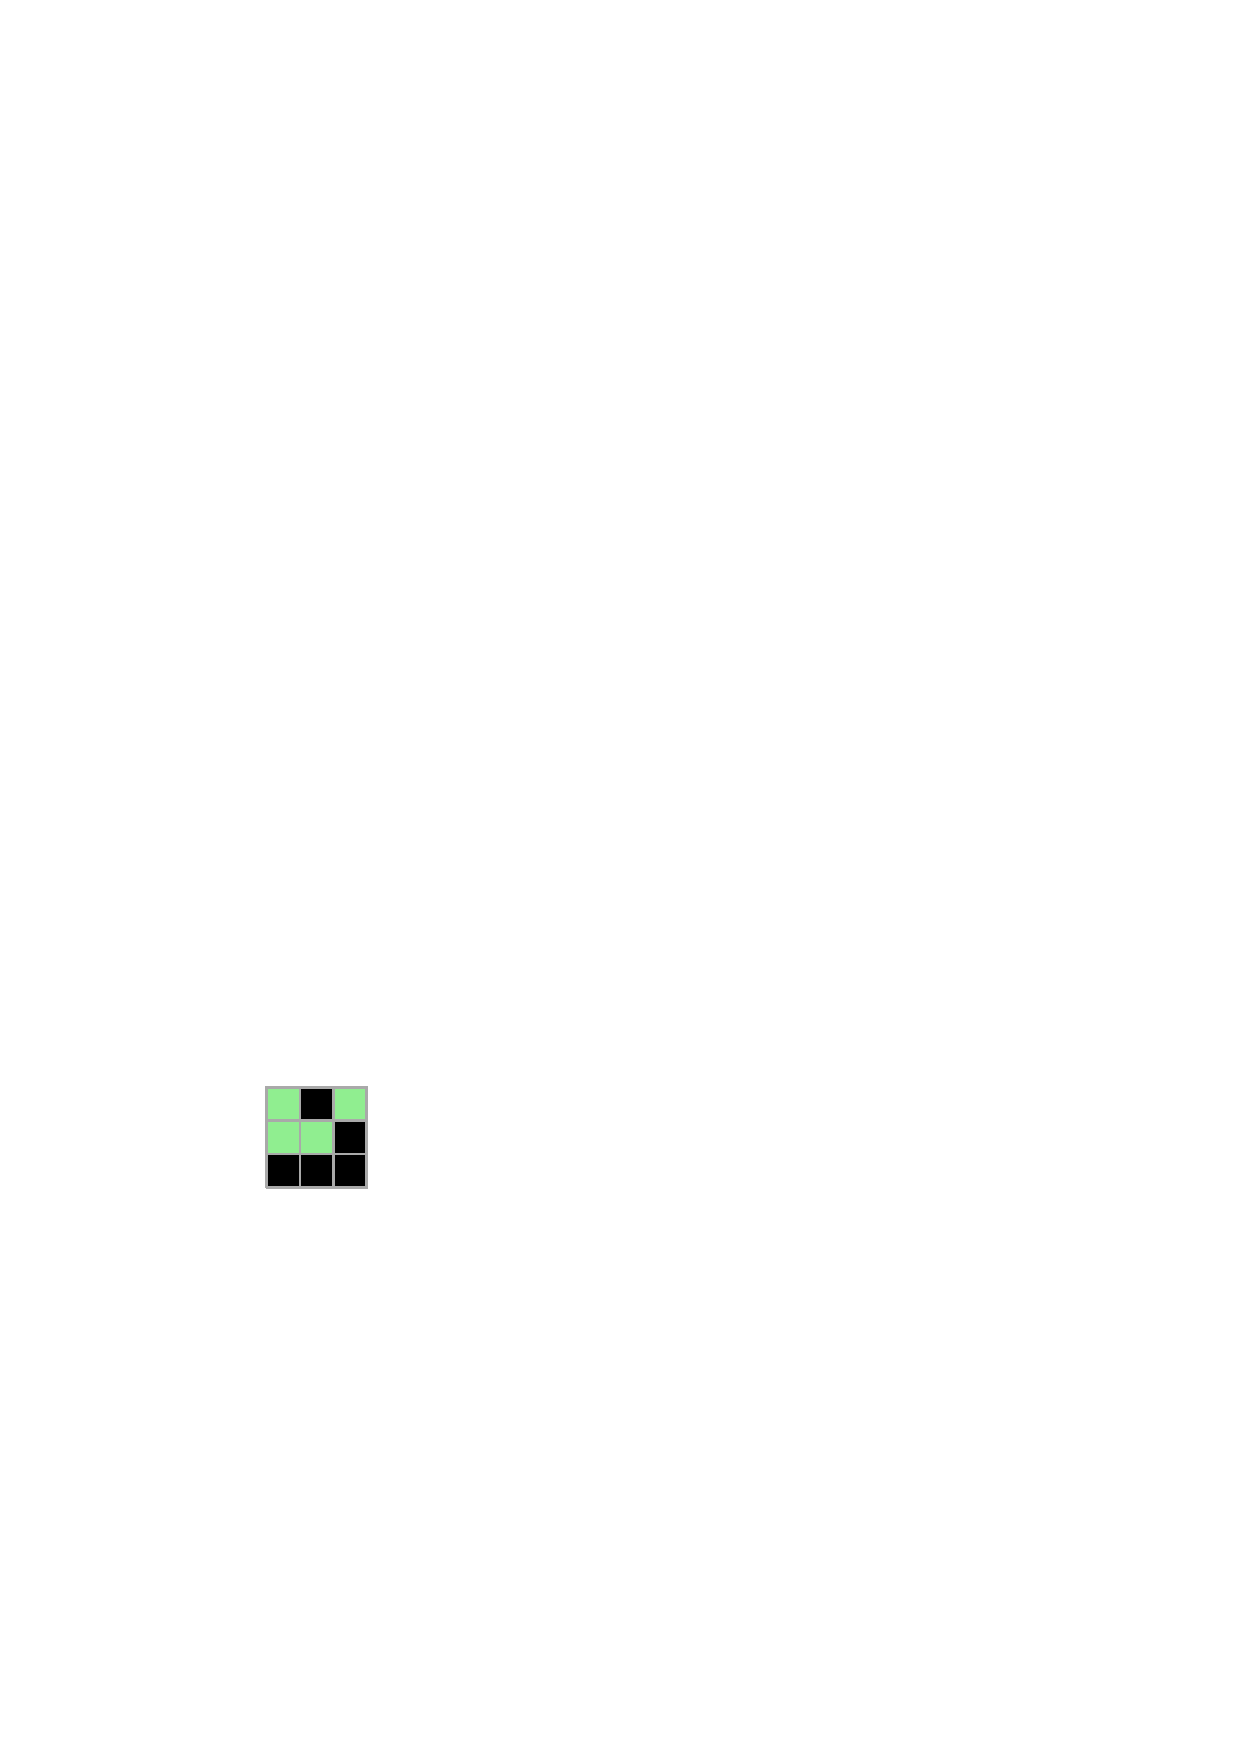
\includegraphics[scale=1]{05_c/figures/gol_init2}
	\hspace{5mm}
	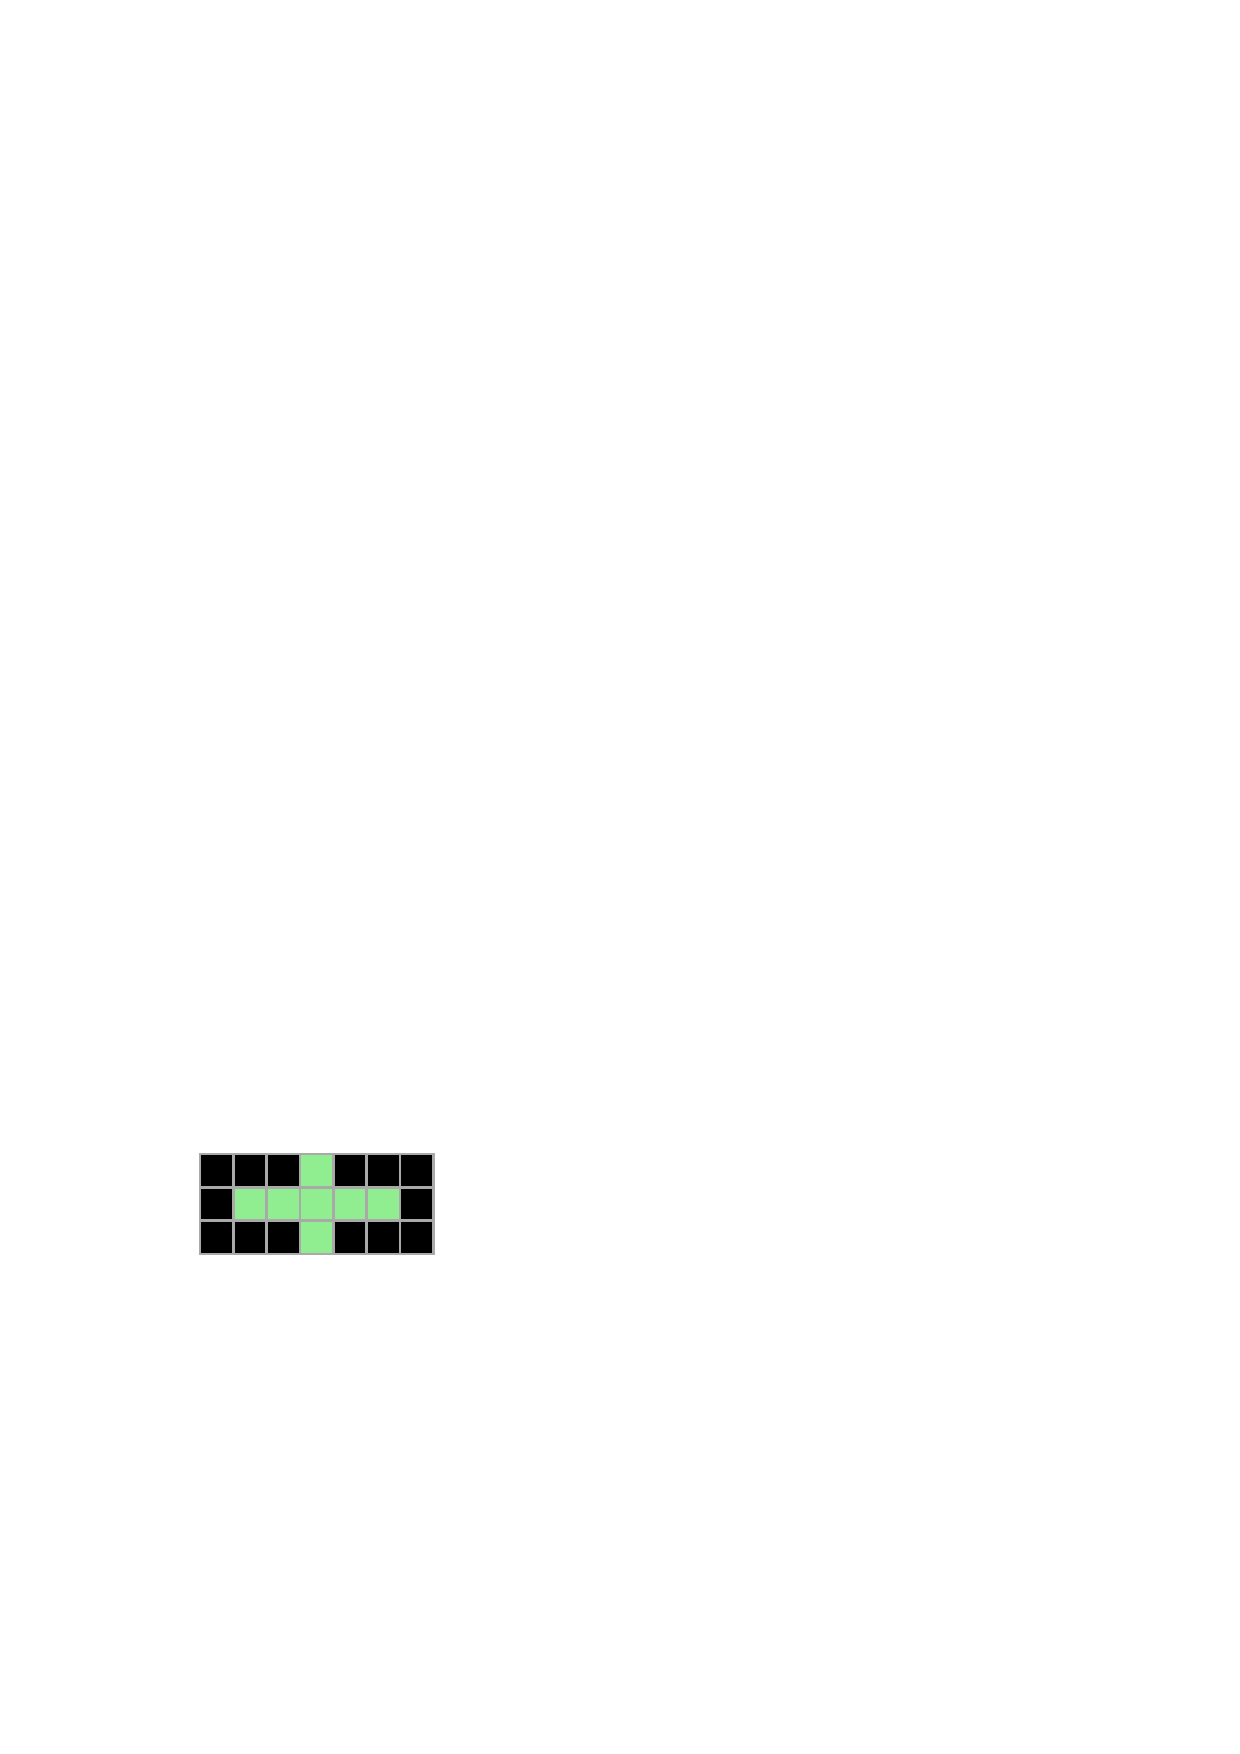
\includegraphics[scale=1]{05_c/figures/gol_init3}
\end{center}
%
\hints{
	\item Da das Spielfeld begrenzt ist, soll es torusförmig aufgebaut werden.
    Das heißt: Alles, was am unteren Rand des Spielfelds verschwindet, kommt oben wieder heraus -- das gleiche gilt für den linken und rechten Rand. 
	\item Verwende als Spielfeld ein mehrdimensionales Array
	\item Ein weiteres mehrdimensionales Array bietet sich an, um die zukünftige Generation erzeugen zu können.
	\item Achte beim torusförmigen Feld unbedingt darauf, dass du nicht über die Grenzen des Spielfelds hinaus zugreifst!
    Das kann zu unvorhersehbarem und schwer zu debuggendem Verhalten des ganzen Displays führen!
}

\subsection*{Vorschlag: Regentropfen}

Das Touch-Display ist ein kleiner Teich;
wenn du eine Stelle mit dem Finger berührst, breitet sich von dort eine konzentrische Welle aus.
Die Geschwindigkeit der Welle kannst du zusätzlich abhängig machen vom ausgeübten Druck.


\subsection*{Weitere Tipps und Vorschläge}
\begin{minipage}{.45\textwidth}
    \begin{center}Asteroids\\
        \href{https://goo.gl/aE7mgC}{https://goo.gl/aE7mgC}
    \end{center}
    \vspace{2ex}
    \begin{center}Pacman\\
        \href{https://goo.gl/kXthKj}{https://goo.gl/kXthKj}
    \end{center}
    \vspace{2ex}
    \begin{center}Labyrinth\\
        \href{https://goo.gl/VCf85t}{https://goo.gl/VCf85t}
    \end{center}
\end{minipage}
\begin{minipage}{.45\textwidth}
	\begin{center}Ausweichspiele à la Hugo\\
        \href{https://goo.gl/Ab8Go2}{https://goo.gl/Ab8Go2}
    \end{center}
    \vspace{2ex}
	\begin{center}Moorhuhn\\
        \href{https://goo.gl/X2xems}{https://goo.gl/X2xems}
    \end{center}
    \vspace{2ex}
	\begin{center}Snake\\
       \href{https://goo.gl/iL2L5M}{https://goo.gl/iL2L5M}
    \end{center}
\end{minipage}

\hints{
\item 
Der folgenden Wiki-Artikel beschreibt, wie man schnell bestehende Bilder in das eigene Projekt einbinden kann: \url{https://github.com/Echtzeitsysteme/tud-cppp/wiki/RGB565-mit-Gimp}.
\item
Quick Start Guide für das Evaluationsboard: \url{http://www.cypress.com/file/290916/download}
\item
PDL Quick Start Guide: \url{http://www.cypress.com/file/307966/download}
\item
Schaltbild des Evaluationsboards: \url{http://www.cypress.com/file/290921/download}
}